\documentclass{beamer}
\usecolortheme{beaver}

\usepackage[utf8]{inputenc} % указывает кодировку документа
\usepackage[T2A]{fontenc} % указывает внутреннюю кодировку TeX 
\usepackage[main=russian,english]{babel} % указывает язык документа
\usepackage{booktabs}
\usepackage{graphicx}
\usepackage{hyperref}
\hypersetup{
     colorlinks   = true,
     citecolor    = blue
}
\usepackage[ruled,vlined]{algorithm2e}
\usepackage{booktabs}
\usepackage{multicol}
\usepackage{lipsum}
\usepackage{mwe}

\title{Люди в масках}
\author{Михаил Сысак}
\institute{Лаборатория финансовых технологий, МФТИ}

\centering
\date{3 июля 2020 г.}
\begin{document}
\setbeamertemplate{caption}{\raggedright\insertcaption\par}
\setbeamerfont{caption}{size=\small}
\setlength{\abovecaptionskip}{-2pt}
\setlength{\belowcaptionskip}{6pt}
\maketitle

%--------------------------------------------------------------------------

\begin{frame}{Постановка задачи}
\begin{itemize}
    \item Люди в солнечных очках, масках, капюшонах
    \item При использовании банкомата затрудняется идентификация
    \item На встрече с представителем может получиться плохое фото для базы
    \item Возможно умышленное использование окклюзий
\end{itemize}
\end{frame}

%--------------------------------------------------------------------------

\begin{frame}{Постановка задачи}
    \begin{enumerate}
        \item Ранжирование закрытий
        \begin{itemize}
            \item Выяснить, какие закрытия влияют сильнее 
            \item Отранжировать окклюзии по этому показателю
        \end{itemize}
        \item Построение модели
        \begin{itemize}
            \item Модель, дающая численную оценку того, насколько закрыто лицо
            \item Предсказать, что идентификация затруднена
        \end{itemize}
    \end{enumerate}
\end{frame}

%--------------------------------------------------------------------------

\begin{frame}{Методы}
Cropped Labeled Faces in the Wild (LFWcrop)

\begin{figure}[h!]
    \centering
    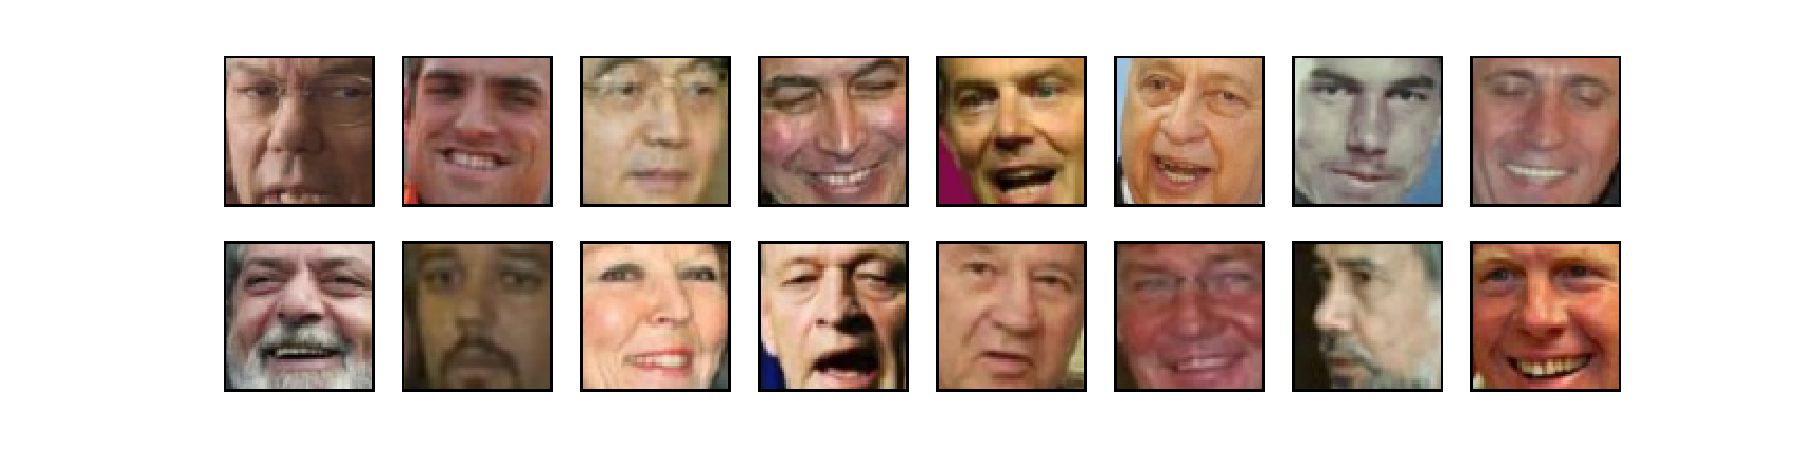
\includegraphics[scale=0.33]{LFWcrop_demo.pdf}
\end{figure}

Шаблоны различных закрытий, их композиции

\begin{figure}[h!]
    \centering
    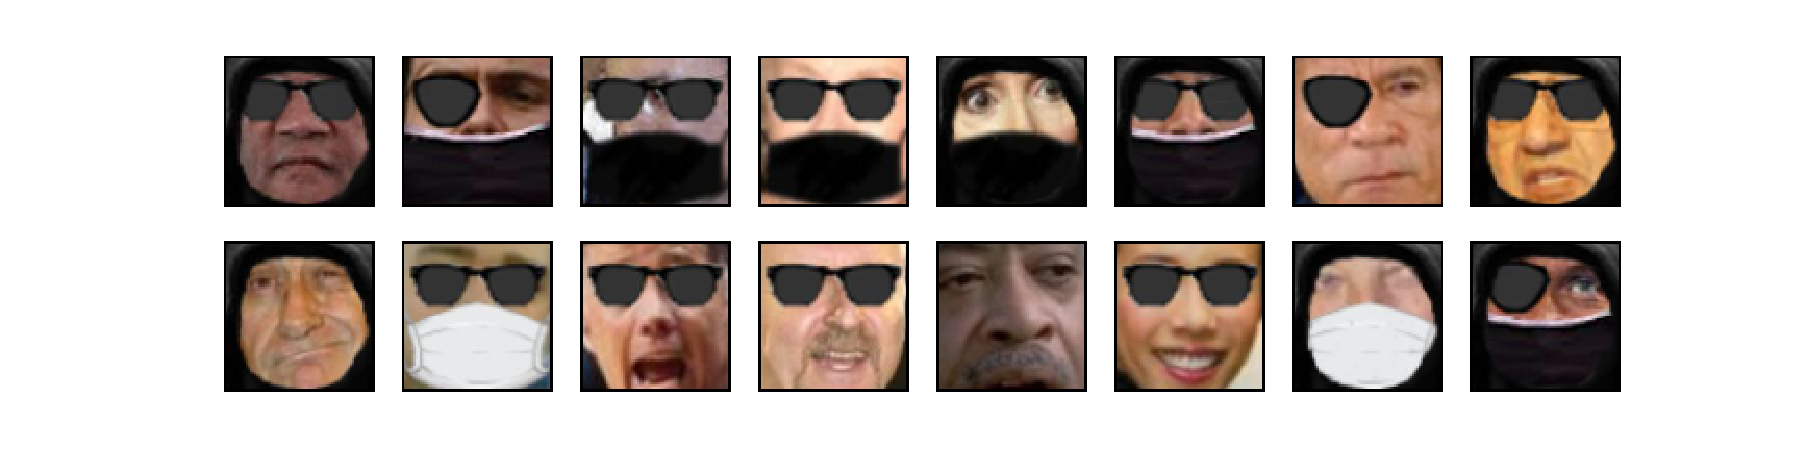
\includegraphics[scale=0.33]{LFWcropObstr_demo.pdf}
\end{figure}

\end{frame}

%--------------------------------------------------------------------------

\begin{frame}{Методы}
\begin{itemize}
    \item Модель Face Recognition из библиотеки dlib
    \item Отображает изображение $150 \times 150$ в вектор размерности $128$
    \item Если расстояние между векторами превышает некоторый порог $T$, то они принадлежат разным людям
\end{itemize}
\end{frame}

%--------------------------------------------------------------------------

\begin{frame}{Методы}
\framesubtitle{Ранжирование закрытий}
\begin{itemize}
    \item Для человека рассматривается кластер его фотографий в латентном пространстве
    \item На фотографии накладывается закрытие, рассматривается второй кластер
    \item Межкластерное расстояние $R$, внутрикластерное расстояние чистых фотографий $r$
    \item Распределение абсолютных $R-r$ и относительных $\dfrac{R-r}{r}$ разностей
    \item Доля случаев, когда человек перестает распознаваться из-за закрытия
\end{itemize}

\end{frame}

%--------------------------------------------------------------------------

\begin{frame}{Результаты}
\framesubtitle{Ранжирование закрытий}
Для каждого закрытия получены два распределения и вероятность затруднения идентификации

\begin{figure}[h!]
    \centering
    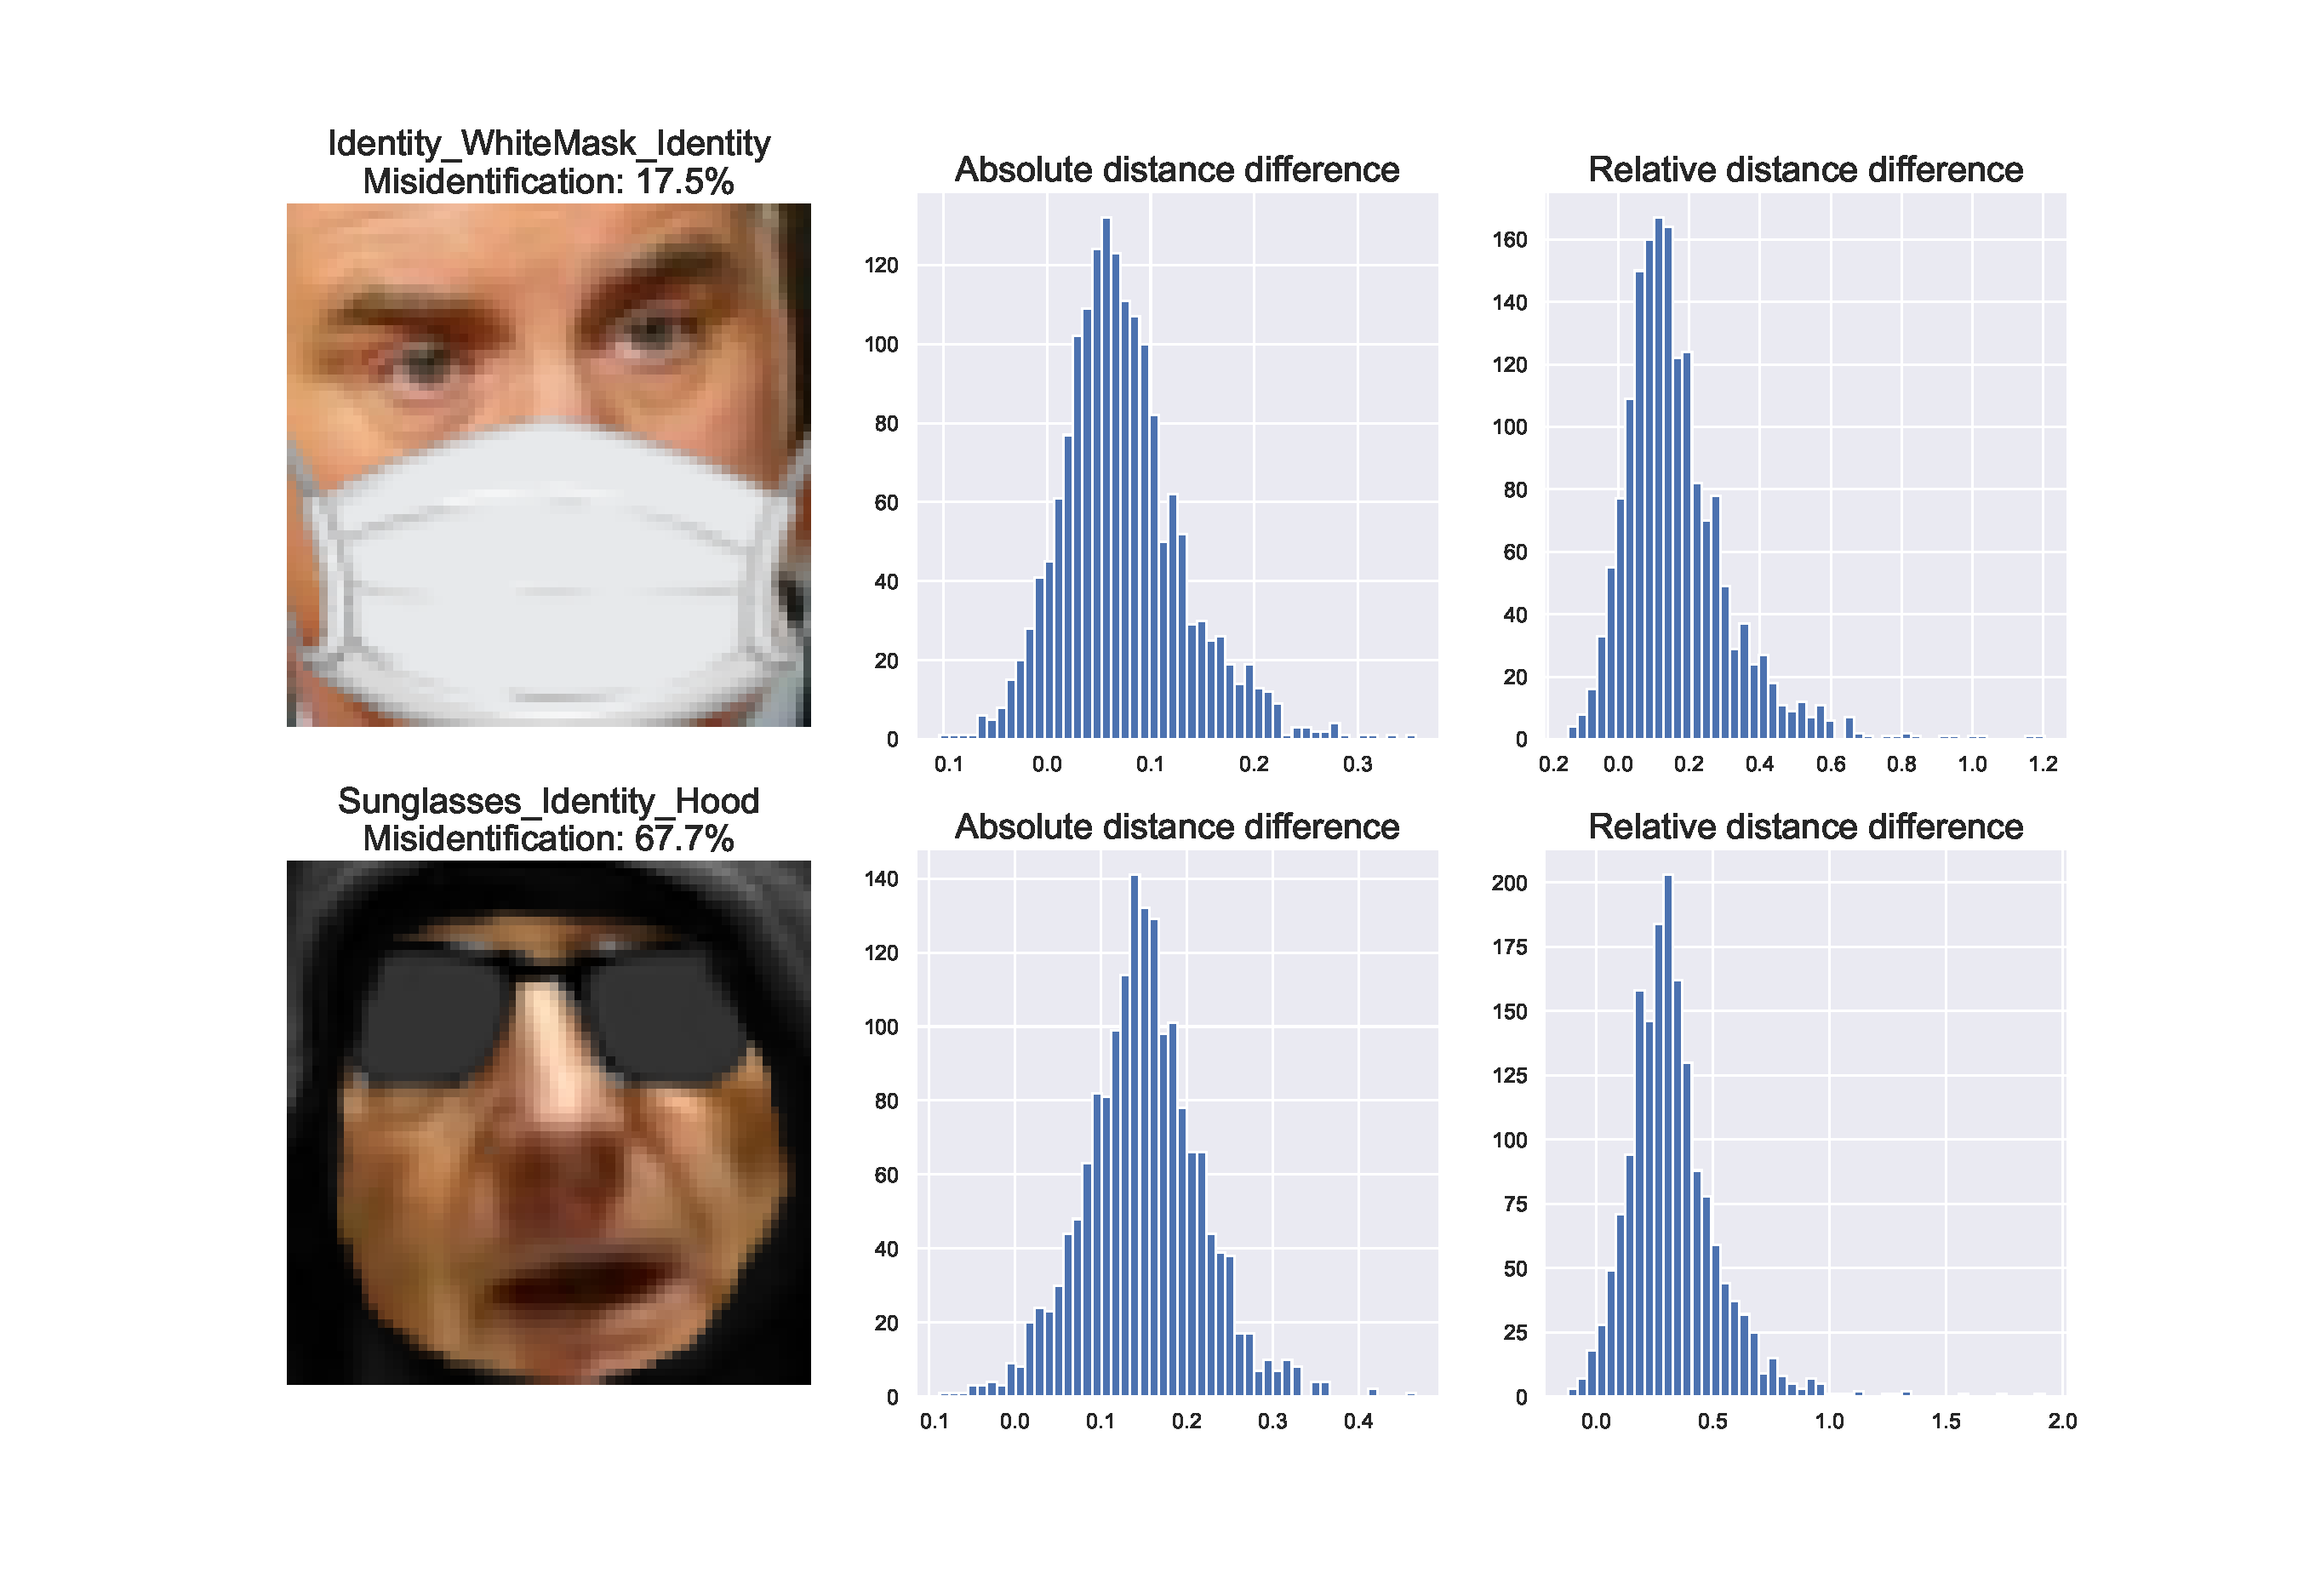
\includegraphics[scale=0.21]{statistics_demo.pdf}
\end{figure}
\end{frame}

%--------------------------------------------------------------------------

\begin{frame}{Результаты}
\framesubtitle{Ранжирование закрытий}
Окклюзии отранжированы по вероятности затрудения идентификации
\begin{columns}

\begin{column}{0.5\textwidth}
\begin{table}[h!]
\centering
\resizebox{0.95\textwidth}{!}{%
\begin{tabular}{lllr}
\toprule
       Eyes &      Mouth &      Head &  ID fault share, \% \\
\midrule
   Identity &   Identity &  Identity &         0.00 \\
   Eyepatch &   Identity &  Identity &        11.87 \\
   Identity &      Scarf &  Identity &        15.51 \\
   Identity &  WhiteMask &  Identity &        17.47 \\
   Identity &   Identity &      Hood &        23.88 \\
   Identity &  BlackMask &  Identity &        26.10 \\
 Sunglasses &   Identity &  Identity &        26.77 \\
   Eyepatch &      Scarf &  Identity &        37.12 \\
   Eyepatch &  WhiteMask &  Identity &        40.85 \\
   Eyepatch &   Identity &      Hood &        45.19 \\
   Identity &      Scarf &      Hood &        52.58 \\
   Eyepatch &  BlackMask &  Identity &        56.39 \\
   \bottomrule
\end{tabular}}
\end{table}
\end{column}

\begin{column}{0.5\textwidth}
\begin{table}[h!]
\centering
\resizebox{0.95\textwidth}{!}{%
\begin{tabular}{lllr}
\toprule
       Eyes &      Mouth &      Head &  ID fault share, \% \\
\midrule
   Identity &  BlackMask &      Hood &        66.57 \\
 Sunglasses &   Identity &      Hood &        67.67 \\
   Eyepatch &      Scarf &      Hood &        70.30 \\
 Sunglasses &  WhiteMask &  Identity &        72.56 \\
   Identity &  WhiteMask &      Hood &        78.71 \\
 Sunglasses &      Scarf &  Identity &        85.22 \\
   Eyepatch &  BlackMask &      Hood &        88.48 \\
 Sunglasses &  BlackMask &  Identity &        89.06 \\
 Sunglasses &      Scarf &      Hood &        94.06 \\
   Eyepatch &  WhiteMask &      Hood &        95.00 \\
 Sunglasses &  WhiteMask &      Hood &        95.88 \\
 Sunglasses &  BlackMask &      Hood &        96.95 \\
 \bottomrule
\end{tabular}}
\end{table}
\end{column}

\end{columns}

\end{frame}

%--------------------------------------------------------------------------

\begin{frame}{Методы}
\framesubtitle{Построение модели}
\begin{itemize}
    \item Даны пары фотографий одного человека $A, B$
    \item Ко второй фотографии применяется окклюзия, получается закрытая фотография $B'$
    \item В качестве метки выступает разность расстояний в латентном пространстве
    $$y = \|B' - A\| - \|B - A\|$$
    \item Строится модель, предсказывающая по закрытой фотографии метку $y$
    \item Архитектура модели~---~MobileNet
\end{itemize}
\end{frame}

%--------------------------------------------------------------------------

\begin{frame}{Методы}
\framesubtitle{Построение модели}
Примеры из обучающей выборки
\begin{figure}[h!]
    \centering
    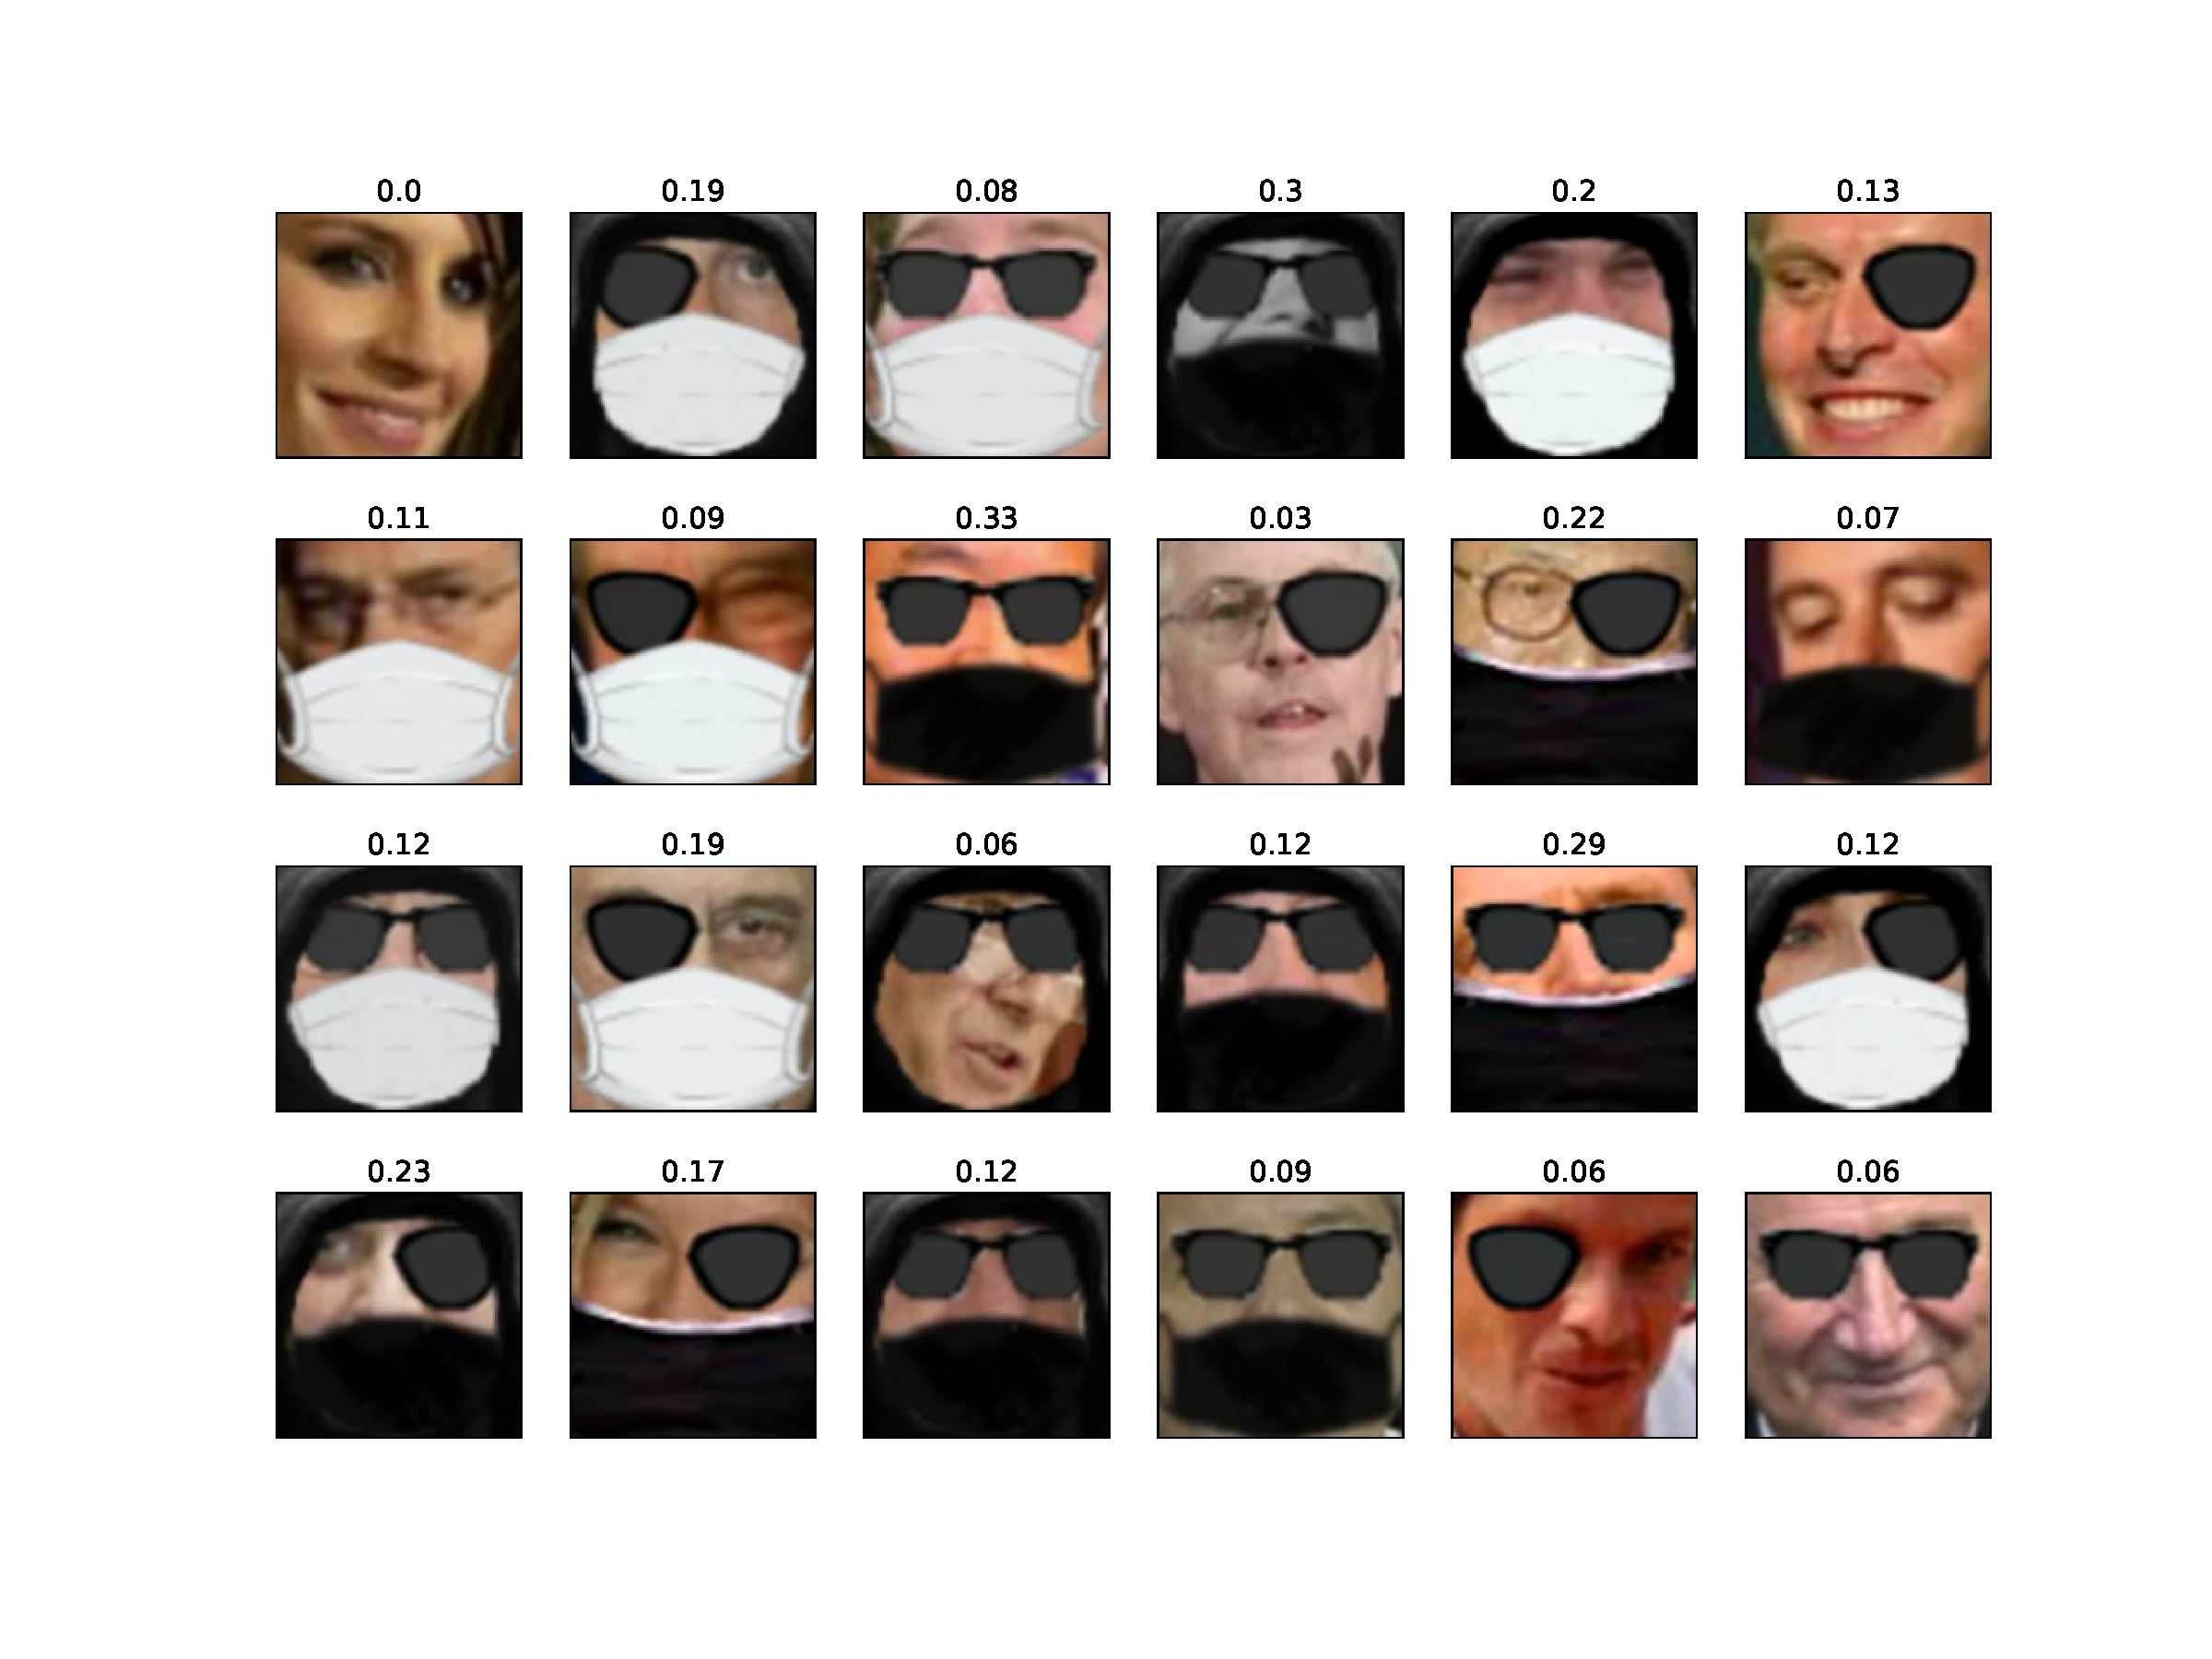
\includegraphics[scale=0.23]{traindata_demo.pdf}
\end{figure}
\end{frame}

%--------------------------------------------------------------------------

\begin{frame}{Методы}
\framesubtitle{Построение модели}
\begin{itemize}
    \item Вычисляется среднее исходных расстояний $$t = \text{mean}(\|B - A\|)$$
    \item По меткам строится бинарный флаг затрудненной идентификации
    $$[y > T-t]$$
    \item По бинарному флагу и пресказаниям сети строится ROC-кривая, вычисляется наилучший threshold $y_0$
    \item Предсказание модели $p$ отображается в вероятность
    $$P(\text{Идентификация затруднена}) = \sigma\left(\dfrac{p}{y_0} - 1\right)$$
\end{itemize}
\end{frame}

%--------------------------------------------------------------------------

\begin{frame}{Результаты}
\framesubtitle{Построение модели}
График остатков ($y - p$ от $y$) и $R^2$ score
\begin{figure}[h!]
    \centering
    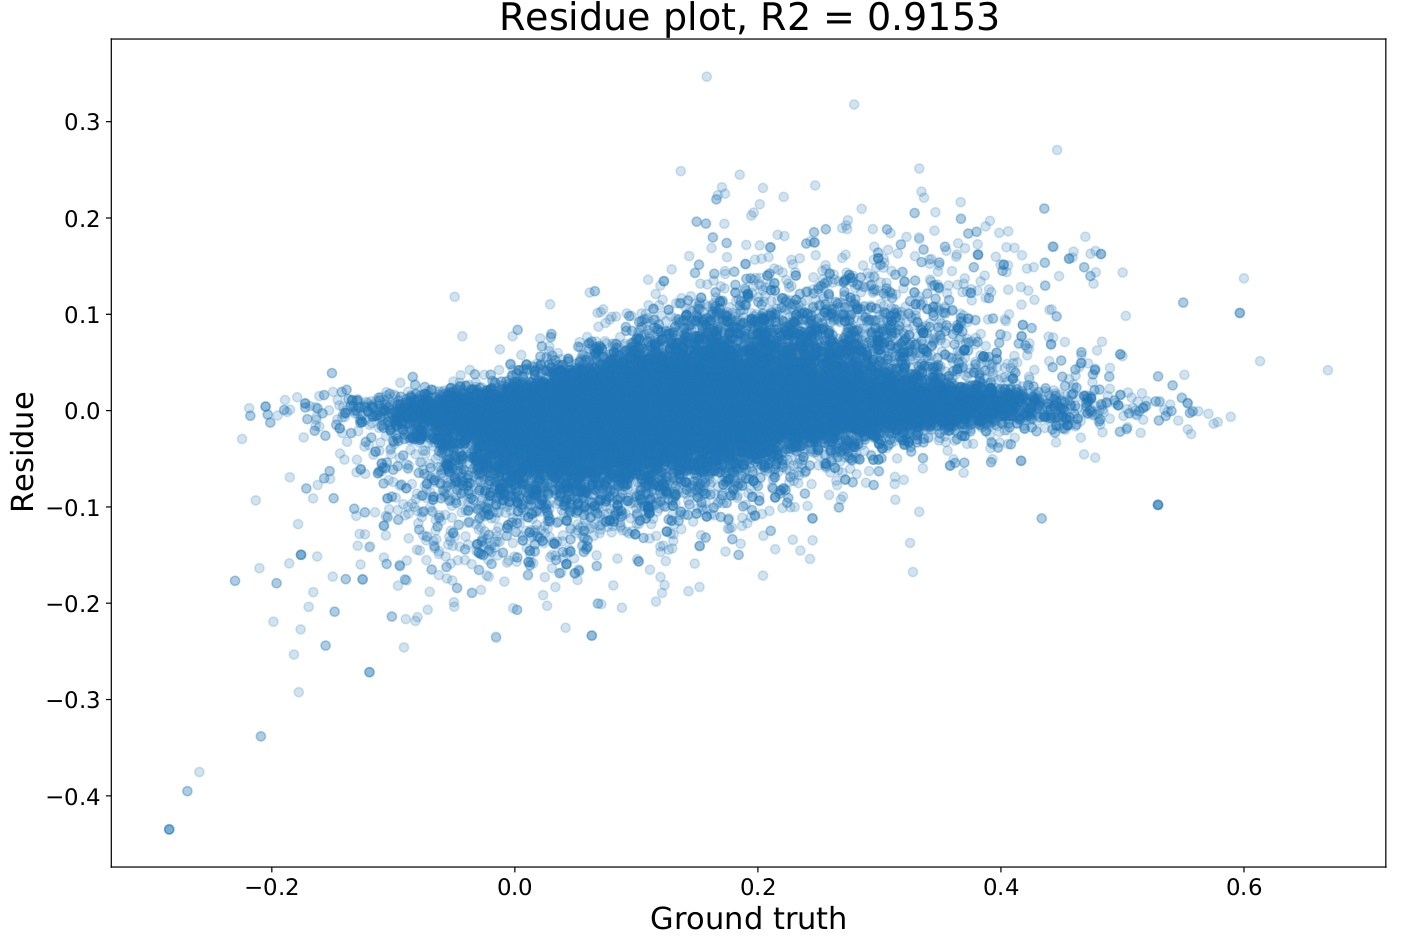
\includegraphics[scale=0.18]{residue_plot.jpg}
\end{figure}
\end{frame}


%--------------------------------------------------------------------------

\begin{frame}{Результаты}
\framesubtitle{Построение модели}
ROC-кривая и ROC-AUC score
\begin{columns}
\begin{column}{0.45\textwidth}
\begin{figure}[h!]
    \centering
    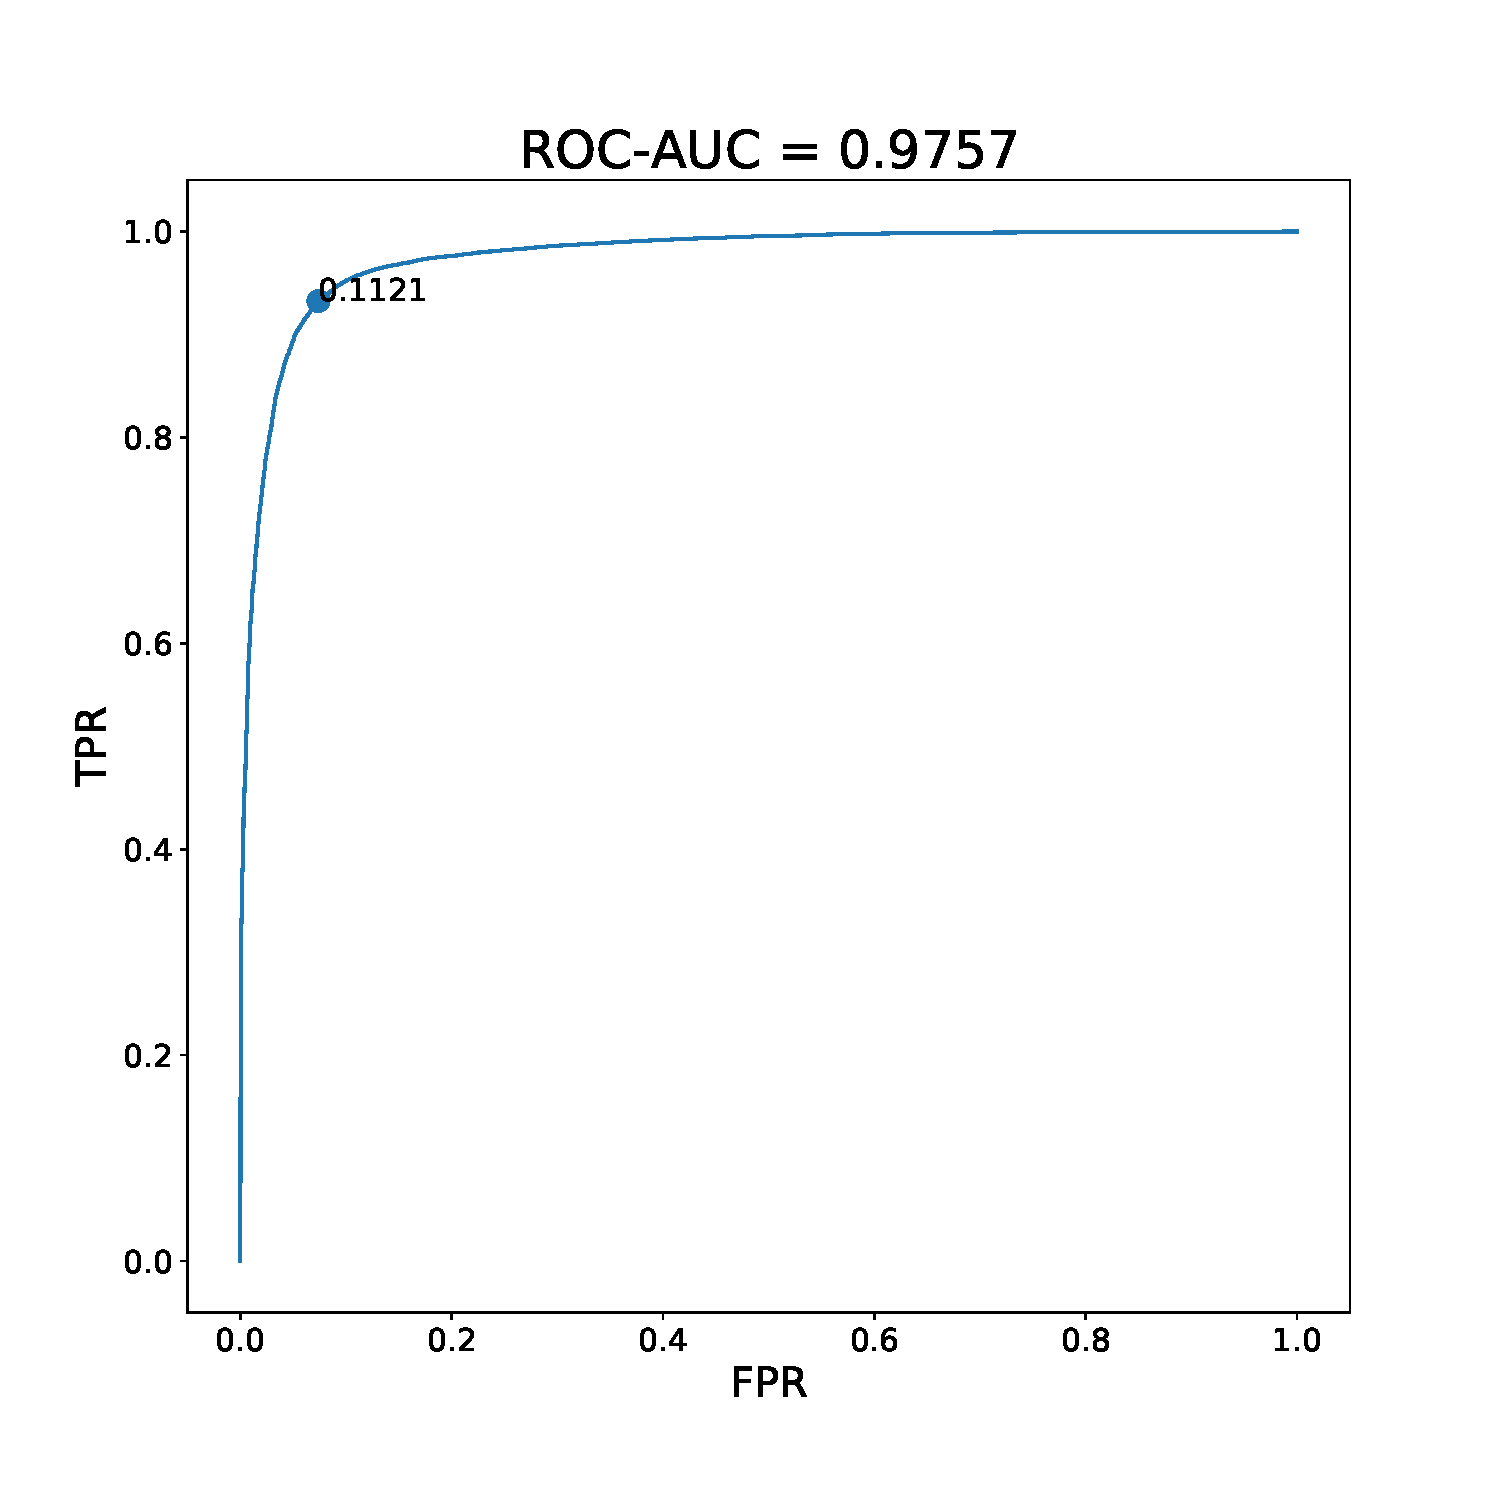
\includegraphics[scale=0.23]{roc_plot.pdf}
\end{figure}
\end{column}
\begin{column}{0.55\textwidth}
\begin{table}[h!]
    \centering
    \begin{tabular}{c|c|c}
   FPR, \% &    TPR, \% &  Threshold \\
\hline
  0.00 &   0.00 &   1.627 \\
  0.09 &  32.40 &    0.220 \\
  0.30 &  42.67 &   0.198 \\
  1.00 &  62.60 &   0.163 \\
  2.99 &  81.44 &   0.133 \\
 10.00 &  95.21 &   0.106 \\
 30.00 &  98.62 &   0.079\\
 \hline
\end{tabular}
\end{table}
\end{column}
\end{columns}
\end{frame}

%--------------------------------------------------------------------------

\begin{frame}{Результаты}
\framesubtitle{Построение модели}
\begin{itemize}
    \item Наилучший threshold: 0.112
    \item FPR при наилучшем threshold: 7.38\%
    \item TPR при наилучшем threshold: 93.24\%
\end{itemize}
Примеры предсказаний модели
\begin{figure}[h!]
    \centering
    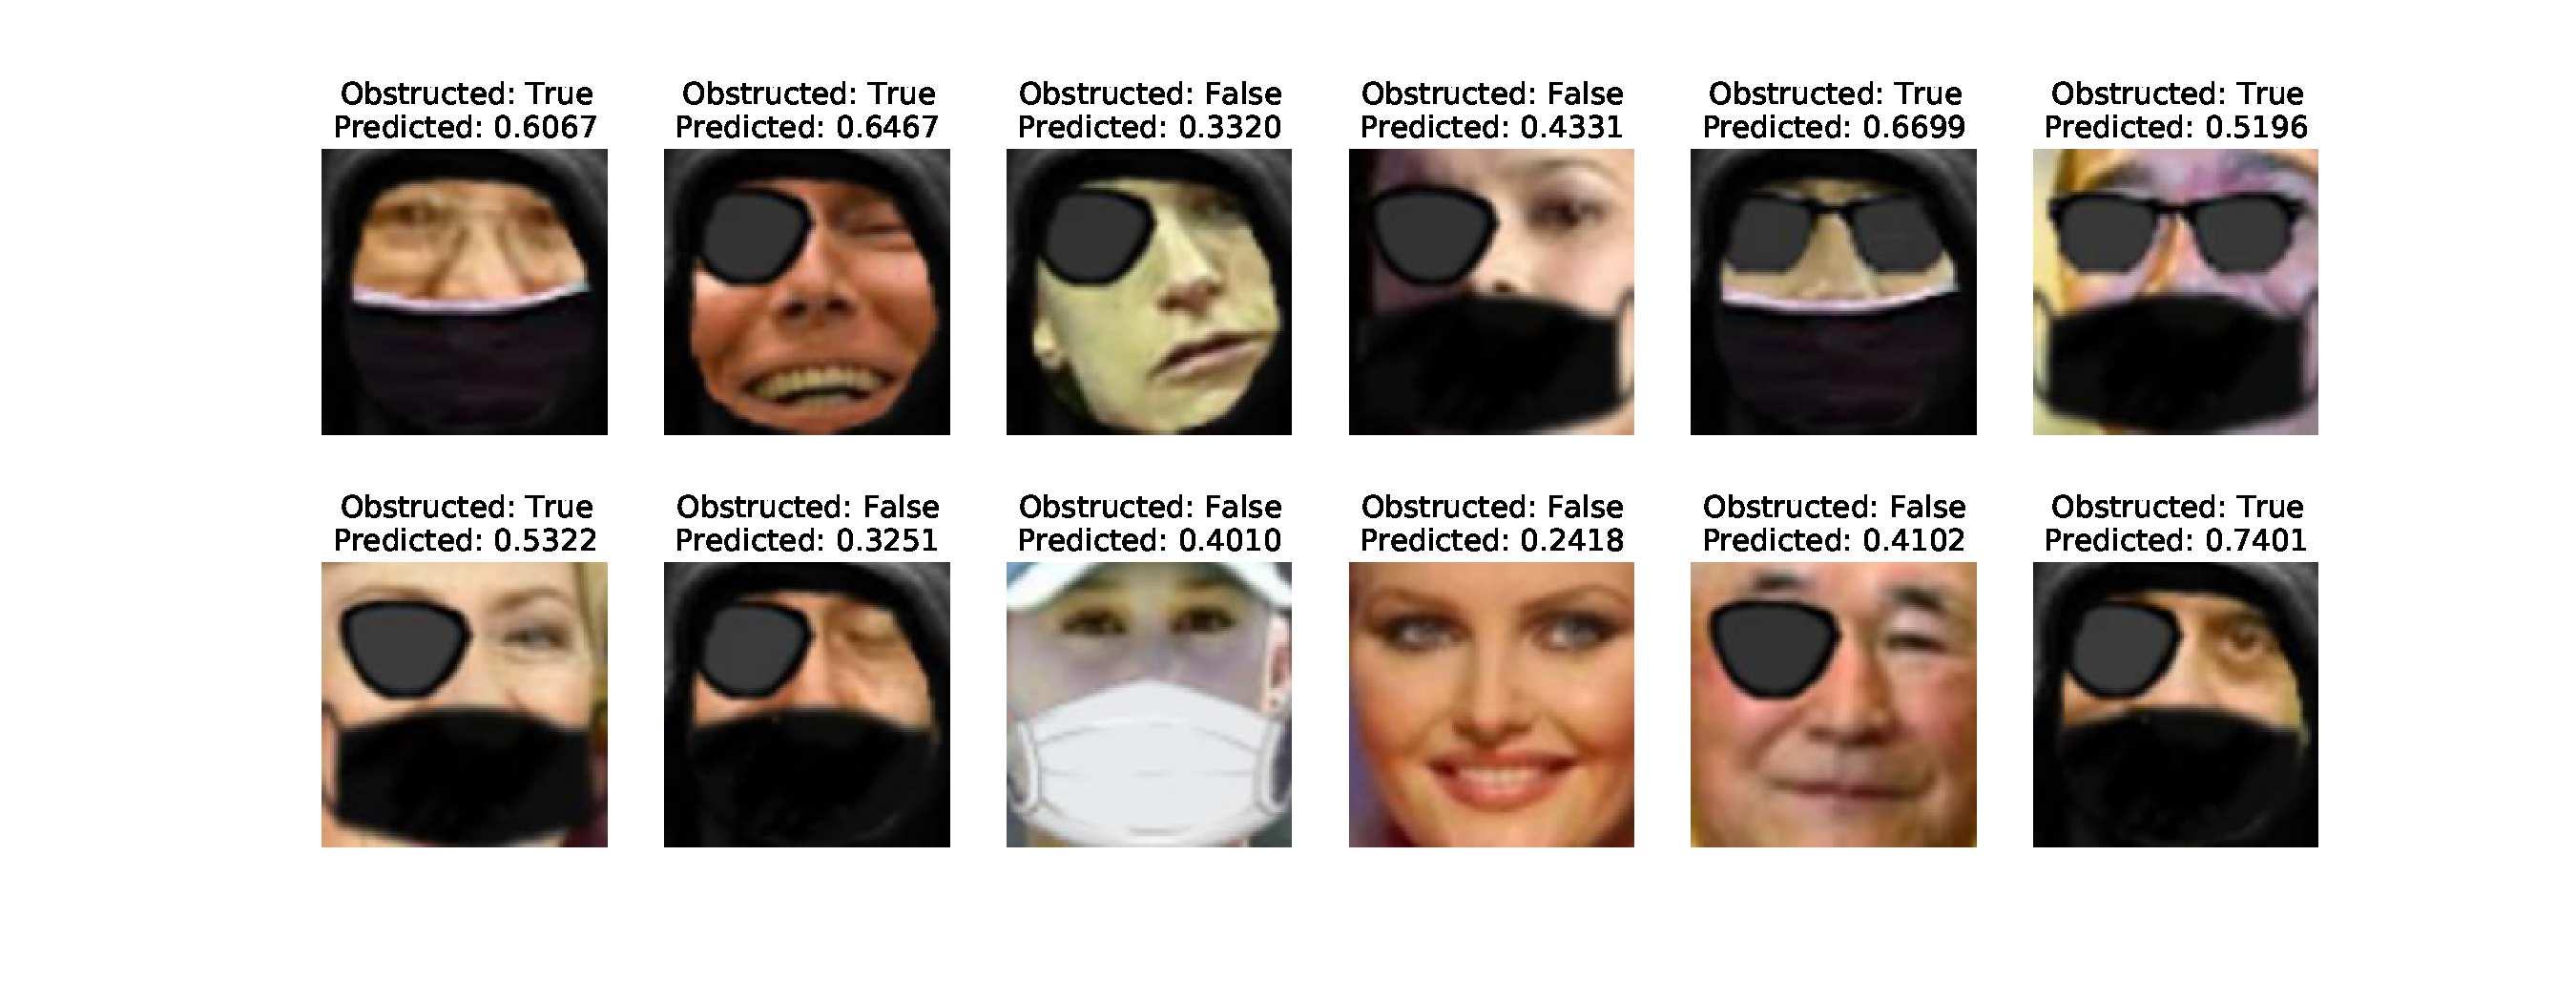
\includegraphics[scale=0.23]{preds_demo.pdf}
\end{figure}
\end{frame}

%--------------------------------------------------------------------------

\begin{frame}{Дальнейшие исследования}
\begin{itemize}
    \item Рассмотрение поворотов лица в качестве окклюзий
    \item Валидация на независимом датасете
    \item Использование более сложных архитектур, более долгое обучение модели
    \item Генерация закрытий по основным точкам лица (лендмаркам)
    \item Проверка работы методов на реальных данных
\end{itemize}
\end{frame}

\end{document}